% !TEX program = xelatex
\documentclass[a4paper]{article}
\usepackage{amsthm}
\usepackage{amssymb}
\usepackage{bm}
\usepackage{mathtools}
\usepackage[x11names]{xcolor}
\usepackage{xparse}
\usepackage{fontspec}
\usepackage{unicode-math}
\setromanfont[Ligatures={Common,Rare}]{DovesType-Regular.otf}
\setsansfont{Andika}
\setmathfont{Asana Math}[Scale=1]
\newfontfamily\TrajanP[Scale=1.0]{TRAJANPRO-REGULAR.OTF}
% \newfontfamily\TrajanP[Scale=1.0]{Tork}

% \usepackage{pstricks}
\usepackage{varwidth}
\usepackage{siunitx}
\usepackage{graphicx}
\usepackage[margin=1.5cm,top=1.5cm]{geometry}
\usepackage[most]{tcolorbox}
\usepackage{pgfplots}
\pgfplotsset{compat=newest}
\tcbuselibrary{skins,xparse,poster,breakable}
% \usetikzlibrary{fadings}
\usetikzlibrary{calc,math, plotmarks, shapes, shapes.geometric, positioning, angles, intersections, quotes, through, patterns, turtle, arrows.meta}
\usetikzlibrary{decorations.markings,backgrounds}
% \usepackage{etoolbox}
\usepackage{tkz-euclide}
% \usepackage{xlop}
% \newcommand\hole[2]{#1}  % for use with xlop
\pagenumbering{gobble}
%%%%%%%%%%%%%%%%%%%%%%%%%%%%%%%%%%%%%%%%%%%%%%%%%%%%%%%%%
\newcommand\markangle[9]{% origin X Y radius radiusmark mark colour opacity
%  % fill red circle offset-from-centre
  \begin{scope}
    \path[clip] (#1) -- (#2) -- (#3);
    \fill[color=#7,fill opacity=#8,draw=black,name path global=pcircle]  % global declaration required otherwise pcircle is not seen by the `named intersections=' lines below.
    (#1) circle (#4);
  \end{scope}
  % middle calculation
  \path[name path=line one] (#1) -- (#2);
  \path[name path=line two] (#1) -- (#3);
  \path[%
  name intersections={of=line one and pcircle, by={inter one}},
  name intersections={of=line two and pcircle, by={inter two}}
  ] (inter one) -- (inter two) coordinate[pos=#9] (place);
  % put mark
  \node at ($(#1)!#5!(place)$) {\scriptsize{#6}};
}
%%%%%%%%%%%%%%%%%%%%%%%%%%%%%%%%%%%%%%%%%%%%%%%%%%%%%%%%
\newcommand\tcircle[6]{% centre coord (x,y), radius, points, radpoint, colour, edge
  \coordinate (O) at (#1,#2); % centre of the circle
  \def\radius{#3}          % radius of the circle
  \def\npts{#4}            % number of the points
  \def\radpt{#5}           % radius of the points
  \colorlet{ptcolour}{#6}  % colour of the points
  % \draw (O) circle (\radius);
  \foreach \numpoint in {1,...,\npts}{
    \fill[ptcolour] (O) ++ (360/\npts*\numpoint:\radius) coordinate (C\numpoint) circle(\radpt);
  }
}

% \newcommand{\condSoln}[2]{\ifcsdef{r@#1}{#2}{}}

% \newcommand\fadingtext[3][]{%
%    \begin{tikzfadingfrompicture}[name=fading letter]
%      \node[text=transparent!0,inner xsep=0pt,outer xsep=0pt,#1] {#3};
%    \end{tikzfadingfrompicture}%
%    \begin{tikzpicture}[baseline=(textnode.base)]
%      \node[inner sep=0pt,outer sep=0pt,#1](textnode){\phantom{#3}};
%      \shade[path fading=fading letter,#2,fit fading=false]
%      (textnode.south west) rectangle (textnode.north east);%
%    \end{tikzpicture}%
% }

\definecolor{JISpurple}{RGB}{89,72,122}
\definecolor{JISivory}{RGB}{241,234,221}
\definecolor{JIStaupe}{RGB}{183,156,154}
\definecolor{PaleGreen}{RGB}{240,255,240} % 'Honeydew'

\AddToHook{shipout/background}{%
    \put (0in,-\paperheight){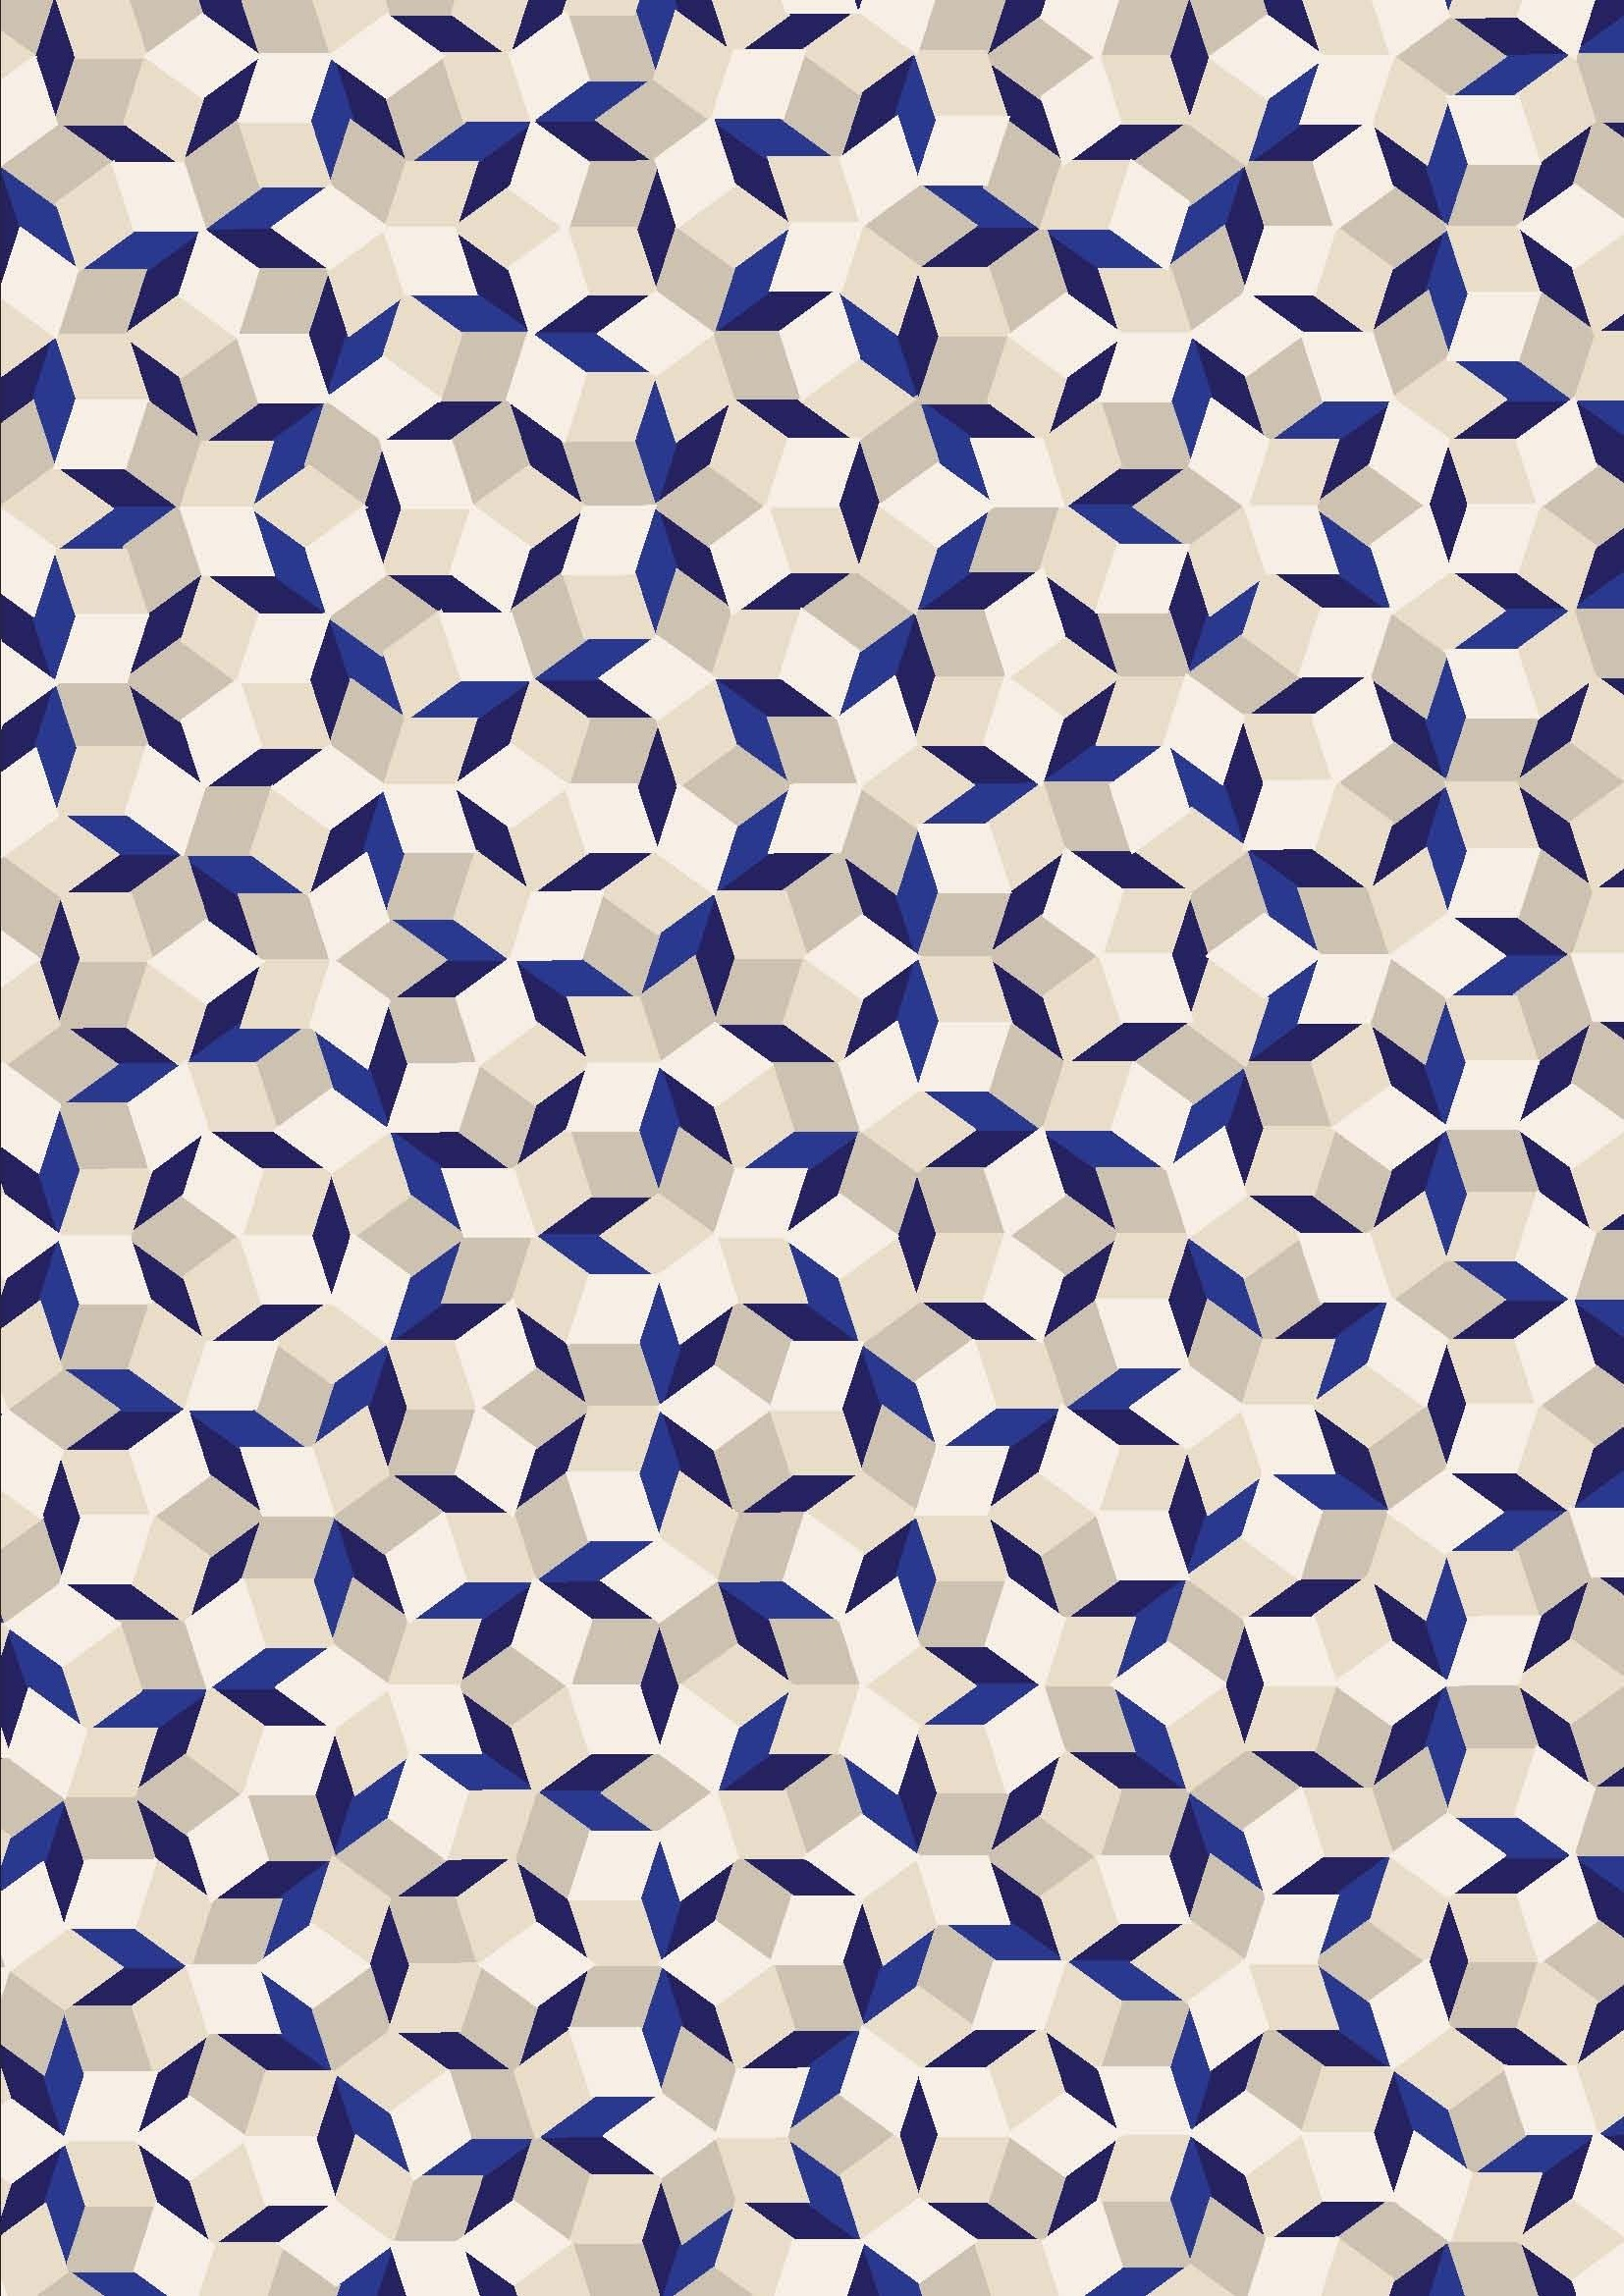
\includegraphics[width=\paperwidth,height=\paperheight]{images/penrose2r.jpg}}%
}

\newcommand\numberthis{\addtocounter{equation}{1}\tag{\theequation}}

\newtcolorbox{MyOuterBox}{%
  enhanced,
  % watermark graphics=images/santa_faces_watermark.jpg,
  % watermark opacity=0.8,
  % watermark zoom=2.0,
  breakable,
  frame style=JISpurple,
  colback=JISivory,
  colframe=JISpurple,
  title={
\includegraphics[width=0.9cm,height=0.9cm]{images/JIS Final Logo FA-02.png}\raisebox{3mm}{\Large{Maths Challenge}\hspace{24em} \Large{\bfseries\sffamily 22}}},
}

\newtcolorbox{MyInnerBox}[2][]{enhanced,%empty,
coltitle=JISpurple,colback=white,
breakable,
fonttitle=\bfseries\sffamily,
attach boxed title to top left={yshift=-1.5mm},
boxed title style={empty, size=small, top=1mm, bottom=0pt},
varwidth boxed title=0.5\linewidth,
frame code={
  \path (title.east|-frame.north) coordinate (aux);
\path[draw=JISpurple, line width=0.5mm, rounded corners,fill=white]
(frame.west) |- ([xshift=-2.5mm]title.north east) to[out=0, in=180] ([xshift=7.5mm]aux)-|(frame.east)|-(frame.south)-|cycle;
},
title={#2},#1}

\newtcolorbox{MyInnerSplitBox}[2][]{enhanced,%empty,
bicolor,sidebyside,sidebyside align=top seam,
righthand width=7.0cm,colbacklower=white,
sidebyside gap=5mm,
breakable,
coltitle=JISpurple,colback=white,
fonttitle=\bfseries\sffamily,
attach boxed title to top left={yshift=-1.5mm},
boxed title style={empty, size=small, top=1mm, bottom=0pt},
varwidth boxed title=0.5\linewidth,
frame code={
  \path (title.east|-frame.north) coordinate (aux);
\path[draw=JISpurple, line width=0.5mm, rounded corners,fill=white]
(frame.west) |- ([xshift=-2.5mm]title.north east) to[out=0, in=180] ([xshift=7.5mm]aux)-|(frame.east)|-(frame.south)-|cycle;
},
title={#2},#1}


\newtcolorbox{MySolutionBox}[1][]{%
  enhanced,
  breakable,
  frame style=JISpurple,
  colback=PaleGreen, colframe=green,
  title={\Large Solution},
  drop fuzzy shadow,
  halign=left,
  #1
}

%%%%%%%%%%%%%%%%%%%%%%%%%%%%%%%%%%%%%%%%%%%%%%%%%%
\newtoggle{SOLUTION}
%%% Uncomment the appropriate line below to show solutions %%%
\toggletrue{SOLUTION}
% \togglefalse{SOLUTION}
%%%%%%%%%%%%%%%%%%%%%%%%%%%%%%%%%%%%%%%%%%%%%%%%%


%%%%%%%%%%%%%%%%%%%%%%%%%%%%%%%%%%%%%%%%%%%%%%%%%%
%%%%%%            DOCUMENT BEGINS           %%%%%%
%%%%%%%%%%%%%%%%%%%%%%%%%%%%%%%%%%%%%%%%%%%%%%%%%%
\begin{document}


  \begin{MyOuterBox}
    \iftoggle{SOLUTION}{Here are the full, or partial solutions.
    }{
      Welcome to this week's Maths Challenge!\\
      Have a go at both questions!\\
      Drop your solution in the box in the staffroom by Tuesday.
    }
       \begin{MyInnerBox}{Year 8 and below}
     Insert the missing parentheses into each equation so that it becomes true when worked out according to the rules of order of operations (e.g. BIDMAS).
     \LARGE{\begin{align*}
       9 + 12 \div 3 + 4 \div 2 + 1\times 2 &= 2\\
       9 + 12 \div 3 + 4 \div 2 + 1\times 2 &= 5\\
       9 + 12 \div 3 + 4 \div 2 + 1\times 2 &= 8\\
       9 + 12 \div 3 + 4 \div 2 + 1\times 2 &= 11\\
       9 + 12 \div 3 + 4 \div 2 + 1\times 2 &= 12\\
       9 + 12 \div 3 + 4 \div 2 + 1\times 2 &= 19
   \end{align*}}
      \iftoggle{SOLUTION}{%conditional output begin
      \begin{MySolutionBox}
     \Large{\begin{align*}
       \shortintertext{First, with no brackets:}
       9 + 12 \div 3 + 4 \div 2 + 1\times 2 &= 17\\
       (9 + 12) \div (3 + 4) \div (2 + 1)\times 2 &= 2\\
       (((9 + 12) \div (3 + 4) \div 2) + 1)\times 2 &= 5\\
       (9 + 12) \div 3 + 4 \div (2 + 1\times 2) &= 8\\
       (9 + 12) \div 3 + 4 \div 2 + 1\times 2 &= 11\\
       9 + (12 \div 3 + 4) \div (2 + 1\times 2) &= 11\\
       9 + 12 \div (3 + (4 \div (2 + 1\times 2))) &= 12\\
       (((9 + (12 \div 3) + 4) \div 2) + 1)\times 2 &= 19
   \end{align*}}
      \end{MySolutionBox}
    }{}%conditional output end
    \end{MyInnerBox}


    \vspace{0.4cm}
          \begin{MyInnerBox}{Year 9 and above}
        Find two rational numbers, both less than ten, whose product is ninety-nine.\par
        A rational number is a fraction \(\frac{a}{b}\), where \(b\neq 0\) and \(a,b\in\mathbb{Z}\), that is, \(a\) and \(b\) are both integers.\par
      \iftoggle{SOLUTION}{%conditional output begin
      \begin{MySolutionBox}
        We are looking for \(\frac{a}{b}\) and \(\frac{c}{d}\) such that
        \begin{align*}
          \frac{a}{b}\times\frac{c}{d} &= 99\\
          \shortintertext{We can try starting with \(c=99\)}
          \frac{a}{b}\times\frac{99}{d} &= 99\\
          \shortintertext{Then we must have}
          \frac{a}{bd} &= 1\\
          \shortintertext{and we must have}
          \frac{a}{b} &< 10,\quad \frac{99}{d} < 10\\
          \shortintertext{Multiplying numerator and denominator by \(999\):}
          \frac{999}{b} \times\frac{99}{999} &= 99\\
          \shortintertext{and then by \(100\):}
          \frac{999}{100}\times\frac{99\times 100}{999} &= 99\\
          \frac{999}{100}\times\frac{9900}{999} &= 99\\
          \shortintertext{Where}
          \frac{999}{100} = 9.99 < 10\qquad &\text{and}\qquad\frac{9900}{999} = 9.\overline{909} < 10
          \intertext{\underline{An alternative way:} Write \(99\) as a product of two of its factors,}
          9\times 11 &= 99\\
          \shortintertext{then multiply by a fraction and its reciprocal,}
          \frac{13}{11}\times 9\quad\times\quad\frac{11}{13}\times 11 &=99\\
          \shortintertext{Notice that we multiply \(9\) by the smaller fraction and \(11\) by the larger.}
          \shortintertext{But,}
          \frac{13}{7}\times 9 & > 10
          \shortintertext{so we need to try smaller fractions:}
          \frac{11}{10}\times 9\quad\times\quad\frac{10}{11}\times 11 &=99
          \shortintertext{but}
          \frac{10}{11}\times 11 &\nless 10
          \shortintertext{trying again:}
          \frac{22}{21}\times 9\quad\times\quad\frac{21}{22}\times 11 &= 99
          \shortintertext{but still \((21\div 22)\times 11 >10\) so we try again,}
          \frac{21}{19}\times 9\quad\times\quad\frac{19}{21}\times 11 &= 999
          \shortintertext{At last!}
          \frac{189}{19} = 9.947\dots < 10\qquad &\text{and}\qquad\frac{209}{21} = 9.952\dots < 10
        \end{align*}
      \end{MySolutionBox}
    }{}%conditional output end
    \end{MyInnerBox}


  \end{MyOuterBox}

%%%%%%%%%%%%%%%%%%%%%%%%%%%%%%%%%%%%%%%%%%%%%%%%%%
\end{document}



